\documentclass[utf8,compress]{beamer}

\usetheme{Warsaw}
\usecolortheme{whale}

\usepackage[francais]{babel}
\usepackage{multicol}

%\newcommand{\slidesubject}{Présentation en \LaTeX}

\title{Développement de services Web JAX-RS pour l’import de données voirie et transport en commun}
\subtitle{\slidesubject}
	\subject{\slidesubject}
\author{Bertrand \textsc{Guerrero}}
\institute{
    Formation professionnelle Concepteur / Développeur \\
    MobiGIS\\
    \vspace{0.8em}
    \emph{- Responsables -} \\
    M.~Christophe \textsc{Lapierre}\\
    M.~Julien \textsc{Lesbegueries}
}
\date{17 Juillet 2015}

%% Définition du répertoire contenant les images
\graphicspath{{images/}}

\logo{
\includegraphics[height=1cm]{logos_mobigis.jpg}}

%% Numérotation des slides :
%% http://texblog.net/latex-archive/plaintex/beamer-footline-frame-number/

%% Solution 1
%\newcommand*\oldmacro{}%
%\let\oldmacro\insertshorttitle%
%\renewcommand*\insertshorttitle{%
%  \oldmacro\hfill%
%  \insertframenumber\,/\,\inserttotalframenumber}

%% Solution 2
\expandafter\def\expandafter\insertshorttitle\expandafter{%
  %\insertshorttitle\hfill%
  \insertframenumber}

\begin{document}

\begin{frame}
\titlepage
\end{frame}

\logo{
\includegraphics[height=1cm]{logos_mobigis.jpg}}

\section{Plan}

\begin{frame}{Plan}
   \begin{multicols}{2}
	\tableofcontents
   \end{multicols}
\end{frame}

%% Un rappel du plan sera affiché à chaque début de section.
\AtBeginSection[]
{
  \begin{frame}<beamer>
    %\frametitle{Plan}
   \begin{multicols}{2}
     \tableofcontents[currentsection,hideothersubsection]
   \end{multicols}
  \end{frame}
}
\section{Présentation de l’entreprise}
\subsection{MobiGIS}
\begin{frame}{MobiGIS}
\begin{block}{Activités}
Société de services en géomatique, et NTIC.\\	
L’activité de MobiGIS est centrée sur les services SIG et l’édition de logiciels. \\
Les clients de MobiGIS sont par exemples des industries, la grande distribution, les collectivités locales, et
les intégrateurs et société de services en ingénierie informatique (SSII). \\
Les logiciels développés permettent de faire des analyses multiples : territoire, pollutions, démographie, etc., d’élaborer des plans de déplacement
urbain et entreprise, d’étudier et de préparer la réorganisation des réseaux multimodaux et la création de nouvelles infrastructures de transport.
\end{block}
\end{frame}
\subsection{Domaine d'application}
\begin{frame}{Domaine d'application}
\begin{block}{Les Systèmes d’Informations Géographiques (SIG)}
Les Systèmes d’Informations Géographiques (SIG) sont des outils informatiques permettant
de représenter et d’analyser toutes les choses qui existent sur terre ainsi que tous les événements
qui s’y produisent. \\
Le SIG appliqué aux transports, peut être utilisé
pour gérer et analyser certaines informations essentielles :\\
— Planification et modélisation des transports\\
— Planification et analyse des itinéraires\\
— Localisation et suivi automatiques des véhicules\\
\end{block}
\end{frame}
\subsection{Références}
\begin{frame}{Références}
\begin{block}{C'est quoi ce document ?}
    Ce document est un exemple de présentation (sous forme de diapositives) faite en LaTeX.
\end{block}
\begin{block}{Où trouver les sources ?}
    Les sources sont disponibles sur mon blog \url{http://blog.hikoweb.net/}.
\end{block}
\begin{block}{Je peux m'en inspirer pour ma propre présentation ?}
    Oui, vous êtes libre d'utiliser les sources comme bon vous semble.
\end{block}
\end{frame}

\AtBeginSection[]
{
  \begin{frame}<beamer>
		\begin{multicols}{2}
     \tableofcontents[currentsection,hideothersubsection]
   \end{multicols}
  \end{frame}
}

\section{Contexte du projet}
\subsection{Projet MobiSAAS}
\begin{frame}{Projet MobiSAAS}
\begin{block}{C'est quoi ce document ?}
    Ce document est un exemple de présentation (sous forme de diapositives) faite en LaTeX.
\end{block}
\begin{block}{Où trouver les sources ?}
    Les sources sont disponibles sur mon blog \url{http://blog.hikoweb.net/}.
\end{block}
\begin{block}{Je peux m'en inspirer pour ma propre présentation ?}
    Oui, vous êtes libre d'utiliser les sources comme bon vous semble.
\end{block}
\end{frame}
\subsection{Cahier des charges}
\begin{frame}{Cahier des charges}
\begin{block}{C'est quoi ce document ?}
    Ce document est un exemple de présentation (sous forme de diapositives) faite en LaTeX.
\end{block}
\begin{block}{Où trouver les sources ?}
    Les sources sont disponibles sur mon blog \url{http://blog.hikoweb.net/}.
\end{block}
\begin{block}{Je peux m'en inspirer pour ma propre présentation ?}
    Oui, vous êtes libre d'utiliser les sources comme bon vous semble.
\end{block}
\end{frame}
\subsection{Contraintes}
\begin{frame}{Contraintes}
\begin{block}{C'est quoi ce document ?}
    Ce document est un exemple de présentation (sous forme de diapositives) faite en LaTeX.
\end{block}
\begin{block}{Où trouver les sources ?}
    Les sources sont disponibles sur mon blog \url{http://blog.hikoweb.net/}.
\end{block}
\begin{block}{Je peux m'en inspirer pour ma propre présentation ?}
    Oui, vous êtes libre d'utiliser les sources comme bon vous semble.
\end{block}
\end{frame}
\subsection{Livrables attendus}
\begin{frame}{Livrables attendus}
\begin{block}{C'est quoi ce document ?}
    Ce document est un exemple de présentation (sous forme de diapositives) faite en LaTeX.
\end{block}
\begin{block}{Où trouver les sources ?}
    Les sources sont disponibles sur mon blog \url{http://blog.hikoweb.net/}.
\end{block}
\begin{block}{Je peux m'en inspirer pour ma propre présentation ?}
    Oui, vous êtes libre d'utiliser les sources comme bon vous semble.
\end{block}
\end{frame}

\AtBeginSection[]
{
  \begin{frame}<beamer>
\begin{multicols}{2}
     \tableofcontents[currentsection,hideothersubsection]
   \end{multicols}
  \end{frame}
}

\section{Gestion de projet}
\subsection{Planning et suivi}
\begin{frame}{Planning et suivi}
\begin{block}{C'est quoi ce document ?}
    Ce document est un exemple de présentation (sous forme de diapositives) faite en LaTeX.
\end{block}
\begin{block}{Où trouver les sources ?}
    Les sources sont disponibles sur mon blog \url{http://blog.hikoweb.net/}.
\end{block}
\begin{block}{Je peux m'en inspirer pour ma propre présentation ?}
    Oui, vous êtes libre d'utiliser les sources comme bon vous semble.
\end{block}
\end{frame}
\subsection{Environnement humain et technique}
\begin{frame}{Environnement humain et technique}
\begin{block}{C'est quoi ce document ?}
    Ce document est un exemple de présentation (sous forme de diapositives) faite en LaTeX.
\end{block}
\begin{block}{Où trouver les sources ?}
    Les sources sont disponibles sur mon blog \url{http://blog.hikoweb.net/}.
\end{block}
\begin{block}{Je peux m'en inspirer pour ma propre présentation ?}
    Oui, vous êtes libre d'utiliser les sources comme bon vous semble.
\end{block}
\end{frame}
\subsection{Objectifs de qualité}
\begin{frame}{Objectifs de qualité}
\begin{block}{C'est quoi ce document ?}
    Ce document est un exemple de présentation (sous forme de diapositives) faite en LaTeX.
\end{block}
\begin{block}{Où trouver les sources ?}
    Les sources sont disponibles sur mon blog \url{http://blog.hikoweb.net/}.
\end{block}
\begin{block}{Je peux m'en inspirer pour ma propre présentation ?}
    Oui, vous êtes libre d'utiliser les sources comme bon vous semble.
\end{block}
\end{frame}

\AtBeginSection[]
{
  \begin{frame}<beamer>
\begin{multicols}{2}
     \tableofcontents[currentsection,hideothersubsection]
   \end{multicols}
	\end{frame}
}

\section{Analyse}
\subsection{Analyse}
\begin{frame}{Analyse}
\begin{block}{C'est quoi ce document ?}
    Ce document est un exemple de présentation (sous forme de diapositives) faite en LaTeX.
\end{block}
\begin{block}{Où trouver les sources ?}
    Les sources sont disponibles sur mon blog \url{http://blog.hikoweb.net/}.
\end{block}
\begin{block}{Je peux m'en inspirer pour ma propre présentation ?}
    Oui, vous êtes libre d'utiliser les sources comme bon vous semble.
\end{block}
\end{frame}
\AtBeginSection[]
{
  \begin{frame}<beamer>
  \begin{multicols}{2}
     \tableofcontents[currentsection,hideothersubsection]
   \end{multicols}
	\end{frame}
}

\section{Conception et codage}
\subsection{Conception}
\begin{frame}{Conception}
\begin{block}{C'est quoi ce document ?}
    Ce document est un exemple de présentation (sous forme de diapositives) faite en LaTeX.
\end{block}
\begin{block}{Où trouver les sources ?}
    Les sources sont disponibles sur mon blog \url{http://blog.hikoweb.net/}.
\end{block}
\begin{block}{Je peux m'en inspirer pour ma propre présentation ?}
    Oui, vous êtes libre d'utiliser les sources comme bon vous semble.
\end{block}
\end{frame}
\subsection{Codage}
\begin{frame}{Codage}
\begin{block}{C'est quoi ce document ?}
    Ce document est un exemple de présentation (sous forme de diapositives) faite en LaTeX.
\end{block}
\begin{block}{Où trouver les sources ?}
    Les sources sont disponibles sur mon blog \url{http://blog.hikoweb.net/}.
\end{block}
\begin{block}{Je peux m'en inspirer pour ma propre présentation ?}
    Oui, vous êtes libre d'utiliser les sources comme bon vous semble.
\end{block}
\end{frame}
\AtBeginSection[]
{
  \begin{frame}<beamer>
  \begin{multicols}{2}
     \tableofcontents[currentsection,hideothersubsection]
   \end{multicols}
  \end{frame}
}

\section{Présentation des éléments les plus significatifs de l’interface de l’application}
\subsection{Résultats}
\begin{frame}{Résultats}
\begin{block}{C'est quoi ce document ?}
    Ce document est un exemple de présentation (sous forme de diapositives) faite en LaTeX.
\end{block}
\begin{block}{Où trouver les sources ?}
    Les sources sont disponibles sur mon blog \url{http://blog.hikoweb.net/}.
\end{block}
\begin{block}{Je peux m'en inspirer pour ma propre présentation ?}
    Oui, vous êtes libre d'utiliser les sources comme bon vous semble.
\end{block}
\end{frame}
\AtBeginSection[]
{
  \begin{frame}<beamer>
\begin{multicols}{2}
     \tableofcontents[currentsection,hideothersubsection]
   \end{multicols}
	\end{frame}
}
\section{Synthèse et conclusion}
\subsection{Bilan professionnel}
\begin{frame}{Bilan professionnel}
\begin{block}{C'est quoi ce document ?}
    Ce document est un exemple de présentation (sous forme de diapositives) faite en LaTeX.
\end{block}
\begin{block}{Où trouver les sources ?}
    Les sources sont disponibles sur mon blog \url{http://blog.hikoweb.net/}.
\end{block}
\begin{block}{Je peux m'en inspirer pour ma propre présentation ?}
    Oui, vous êtes libre d'utiliser les sources comme bon vous semble.
\end{block}
\end{frame}
\subsection{Bilan personnel}
\begin{frame}{Bilan personnel}
\begin{block}{C'est quoi ce document ?}
    Ce document est un exemple de présentation (sous forme de diapositives) faite en LaTeX.
\end{block}
\begin{block}{Où trouver les sources ?}
    Les sources sont disponibles sur mon blog \url{http://blog.hikoweb.net/}.
\end{block}
\begin{block}{Je peux m'en inspirer pour ma propre présentation ?}
    Oui, vous êtes libre d'utiliser les sources comme bon vous semble.
\end{block}
\end{frame}


%\begin{frame}{La page la plus simple}
%C'est simple, il n'y a que du texte.
%
%Quae feminas feminas poterat pedibus ter quocumque nixus usque usque oculos exprimunt nixus quocumque tergentes iactari nixus taedium simulacra tergentes.
%\end{frame}
%
%\begin{frame}[containsverbatim]{Les blocs}
%\begin{block}{Bloc normal}
     %C'est un joli bloc bleu.
%\end{block}
%\begin{exampleblock}{Bloc exemple}
     %Le vert signifie que c'est un exemple.
%\end{exampleblock}
%\begin{alertblock}{Bloc alerte}
     %Attention c'est rouge !
%\end{alertblock}
%\end{frame}
%
%\subsection{Une autre sous-section}
%
%\begin{frame}{Juste une image}
%\begin{figure}[h]
    %\center
    %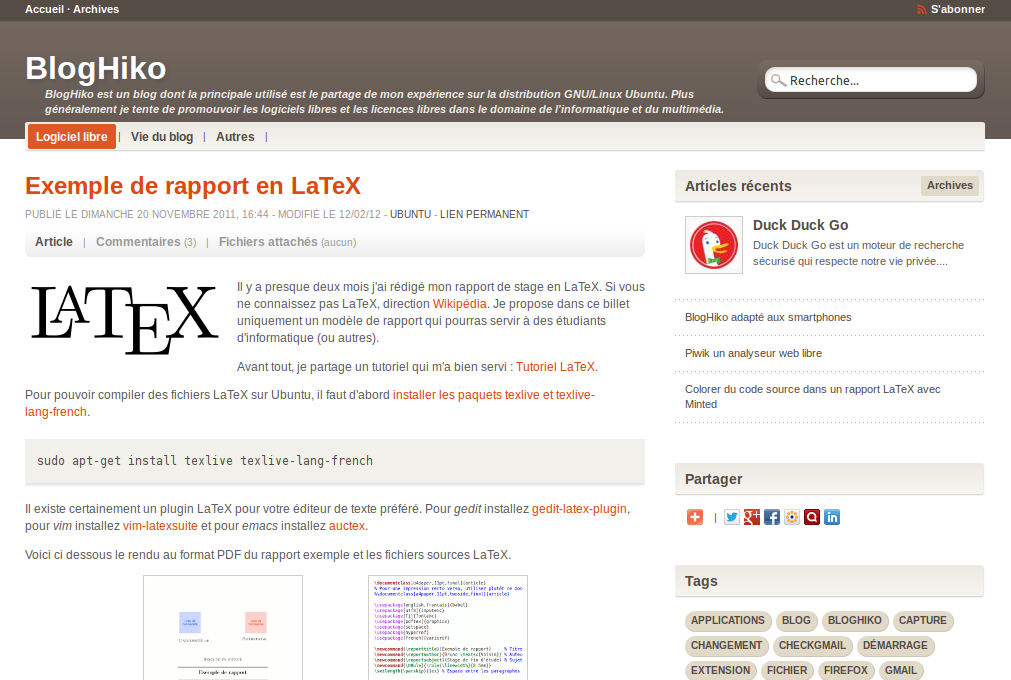
\includegraphics[width=\textwidth]{bloghiko.png}
%\end{figure}
%\end{frame}
%
%
%\section{Deuxième section}
%
%\subsection{C'est pas fini}
%
%\begin{frame}{Liste}
%\begin{itemize}
    %\item Une simple liste,
    %\item avec deux éléments.
%\end{itemize}
%\begin{block}{Implication}
    %\begin{itemize}
    %\item cause
    %\item[$\Rightarrow$] conséquence
    %\end{itemize}
%\end{block}
%\end{frame}
%
%\begin{frame}{Plus compliqué}
%\begin{columns}
%\begin{column}{0.7\textwidth}
    %Cette page est constituée de\dots
    %\begin{itemize}
    %\item deux colonnes ;
    %\item un liste dans la première colonne ;
    %\item une image dans la deuxième colonne ;
    %\item un bloc.
    %\end{itemize}
%\end{column}
%\begin{column}{0.3\textwidth}
    %\begin{figure}[h]
        %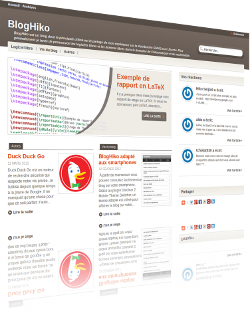
\includegraphics[width=3cm]{bloghiko-reflet3d.png}
    %\end{figure}
%\end{column}
%\end{columns}
%\vspace{1em}
%\begin{block}{Le bloc}
    %Ut eum praeceptum possemus fuit diligendo aliquando diligentiam ut 
    %fuit hoc quam inimicitiarum possemus praeceptum.
%\end{block}
%\end{frame}
%
%
\section{Conclusion}

\begin{frame}{Conclusion}
    Vous pouvez faire des diapositives très professionnelles en toute simplicité.
\end{frame}

\end{document}

